%\section{Diagrama} \label{sec:uml-domain-model}

\begin{figure}[ht]
	\label{tab:uml-domain-model}
	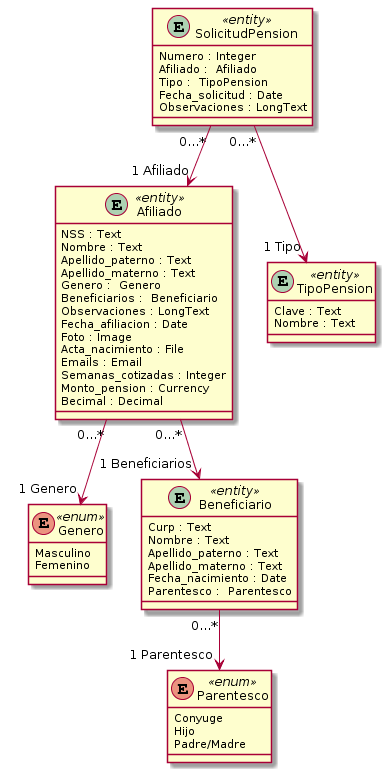
\includegraphics[width=0.5\textwidth]{uml-diagrams/domain-model.png}
	\caption{Modelo de Dominio}
\end{figure}

\section{Descripción de las Entidades de Negocio} \label{sec:entity-description}

\begin{table}[ht]
	\caption{Entidades del Modelo de Dominio}
	\label{tab:entities}
	%\resizebox{\textwidth}{!}{
	\begin{center}
	\begin{tabular}{ l l }
		\hline
		\textbf{Entidad} & \textbf{Descripción} \\
		\hline
		Solicitud Pensión & Información de la Solicitud de Pensión derivada del derecho de un Afiliado al IMSS. \\
		\hline
	\end{tabular}
	\end{center}
	%}
\end{table}

\section{Campos por Entidad de Negocio} \label{sec:entity-fields}

\begin{table}[h]
	\caption{Entidad de Negocio: Solicitud Pensión}
	\label{tab:fields-solicitudpension}
	%\resizebox{\textwidth}{!}{
	\begin{center}
	\begin{tabular}{ l l l l }
		\hline
		\textbf{Campo} & \textbf{Tipo} & \textbf{Restricciones} & \textbf{Descripción} \\
		\hline
		Número & Integer & Required: true & Número de la Solicitud generado automáticamente. \\
		\hline
	\end{tabular}
	\end{center}
	%}
\end{table}
